\documentclass[12pt]{article}
\usepackage[a4paper, inner=1.5cm, outer=3cm, top=2cm,bottom=3cm, bindingoffset=1cm]{geometry}
\usepackage[english]{babel}
\usepackage[utf8x]{inputenc}
\usepackage{amsmath}
\usepackage{tikz}
\usepackage[maxfloats=256]{morefloats}
\usepackage{booktabs}
\usepackage{graphicx}
\usepackage{hyperref}
\usepackage{pdflscape}
\usepackage{adjustbox}
\graphicspath{ {./images/} }
\usepackage{capt-of} 
\usepackage{listings}
\usepackage{xcolor}
\usepackage{setspace}
\definecolor{codegreen}{rgb}{0,0.6,0}
\definecolor{codegray}{rgb}{0.5,0.5,0.5}
\definecolor{codepurple}{rgb}{0.58,0,0.82}
\definecolor{backcolour}{rgb}{0.95,0.95,0.92}
 
\lstdefinestyle{mystyle}{
    backgroundcolor=\color{backcolour},   
    commentstyle=\color{codegreen},
    keywordstyle=\color{magenta},
    numberstyle=\tiny\color{codegray},
    stringstyle=\color{codepurple},
    basicstyle=\ttfamily\footnotesize,
    breakatwhitespace=false,         
    breaklines=true,                 
    captionpos=b,                    
    keepspaces=true,                 
    numbers=left,                    
    numbersep=5pt,                  
    showspaces=false,                
    showstringspaces=false,
    showtabs=false,                  
    tabsize=2
}
 
\lstset{style=mystyle}
 
\begin{document}
\begin{titlepage}
\newcommand{\HRule}{\rule{\linewidth}{0.5mm}} 
\center
\doublespacing
\textbf{\Huge MACHINE LEARNING FOR PREDICTING DIABETES MELLITUS}
\\
\singlespacing
\Large
\vspace{3cm}
A project report submitted in partial fulfilment of the requirement for the degree of\\
\vspace{1cm}
\textbf{Bachelor in Science\\In\\Computer Science}
\\by\\
\Large
Alexander Roque Rodrigues
\\
\vspace{1cm}
under the supervision of
\vspace{1cm}
\\
Ashweta Fondekar
\\
\textbf{PARVATIBAI CHOWGULE COLLEGE OF ARTS \& SCIENCE AUTONOMOUS}
\\June 2019
\end{titlepage}

%declaration
\newpage
\vspace{15cm}
\begin{center}

\textbf{Declaration by Candidate}\\

I declare that this project report has been prepared by me and to the best of my
knowledge, it has not previously formed the basis for the award of any diploma or degree by
any other University.



\end{center}
\newpage
\vspace{15cm}
\begin{center}
\textbf{Certificate by Supervisor}\\
Certified that the Project Report is a record of work done by the candidate himself/herself/themselves under my guidance during the period of study and that to the best of my knowledge, it has not previously formed the basis of the award of any degree or diploma of any other University.\\
\vspace{5cm}
Ashweta Fondekar\\

Project Supervisor
\end{center}
\newpage

\textbf{Work Record}


\newpage
\section{Acknowledgements}

\newpage
\tableofcontents
\newpage
\listoffigures
\newpage
\listoftables
\newpage


\begin{abstract}
Diabetes Mellitus is a disease that prevents the body from properly expanding the
energy stored from the food consumed. The purpose of this project was to select
machine learning algorithms that are able to predict or classify a person as diabetic
or healthy based on the legacy data. The algorithms compared were KNN
Classifier, Logistic Regression, Decision Tree Classifier, Random Forest
Classifier, Gradient Boosting Classifier, Support Vector Classifier and the
Multi-Layered Perceptron. From all the above the Multi-Layered Perceptron gave
an accuracy of prediction on the dataset as ~79.70\%. To improve the performance
of the classifier, I have considered new features deduced from the currently
existing feature set a re-trained the classifier on the new dataset that I generated,
which is now able to classify the subject as diabetic or healthy with a new accuracy
of ~93.10\%. A significant change which boosted the accuracy by 13.4\%. After
selection of the algorithm I further advanced the platform of cluster computing to
deploy the algorithm onto and generate predictions in without any human
interference (apart from entering the data itself) ​ and also made the data available
to the users via an easy to use web application which gives them access to the
observations then stored in the database after being predicted by the algorithm
deployed on the nodes.
\end{abstract}
\onehalfspacing
%\doublespacing


\section{Introduction}
In recent days, there has been a sharp increase in the cases of diabetes mellitus. Diabetes mellitus is on the rise amongst many people and the rate of contracting this lifestyle disease could be reduced significantly if proper measures and precautions were to be instilled amongst people the number of people can be reduced.

Machine learning is a growing field in computer science. With the development and introduction of many algorithms the prediction and accuracy of the predictions itself has improved substantially. Machine learning and healthcare systems are also becoming increasingly popular in the healthcare sector.

The project encompasses the qualities of Remote Patient Monitoring (RPM) and Clinical Decision Support (CDS). RPM provides medical facilities that have the ability to transmit patient data to healthcare professionals who might very well be halfway around the world. RPM can monitor blood glucose levels and blood pressure. It is particularly helpful for patients with chronic conditions such as type 2 diabetes, hypertension, or cardiac disease. Data collected and transmitted via PRM can be used by a healthcare professional or a healthcare team to detect medical events such as stroke or heart attack that require immediate and aggressive medical intervention. Data collected may be used as part of a research project or health study. RPM is a life-saving system for patients in remote areas who cannot access face-to-face health care. CDS analyzes data from clinical and administrative systems. The aim is to assist healthcare providers in making informed clinical decisions. Data available can provide information to medical professions who are preparing diagnoses or predicting medical conditions like drug interactions and reactions. CDS tools filter information to assist healthcare professionals in caring for individual clients. 

The objective of this project is to create a  system that is able to use the machine learning algorithms and predict the outcome of the parameters entered into the algorithm and help the patient draw a conclusion whether or not he/she has the same traits exhibited by similar patients that have diabetes. Also the system should have a UI that is capable of displaying the data of the patients to the doctor and to the patients themselves for further interpretation.

\newpage
\section{Software Requirements}
The main function of this project is to enable the doctors to advise their patients with the help of the prediction software. The system should be accessible to the patient as well as the doctor, therefore it should have a web interface for the two parties to interact with.

\subsection{Functionalities for Doctors}
As an owner of a doctors account a doctor should be able to:
\begin{itemize}
\item Add new observations for the machine learning algorithm to predict.
\item Analyse the patients previous records.
\item Have a dashboard for patient performance monitoring.
\end{itemize}

\subsection{Functionalities for Patients}
As the patient, one should be able to:
\begin{itemize}
\item Should be able to see the predicted risk of developing diabetes.
\item Should be able to view historic data.
\end{itemize}

\subsection{Functionalities for Master Nodes}
As the master nodes:
\begin{itemize}
\item Control chunk size.
\item Remotely update the slave nodes.
\item Check the status of nodes.
\item Control the SQL database.
\end{itemize}

\subsection{Functionalities for Slave Nodes}
\begin{itemize}
\item Should have the machine learning algorithm tuned as per specifications.
\item Remote update should be possible.
\item Remote access should be possible.
\end{itemize}

\newpage
\section{Hardware Requirements}
\subsection{Raspberry Pi}

According to raspberrypi.org, the Raspberry Pi 3 Model B is the earliest model of the third-generation Raspberry Pi. It replaced the Raspberry Pi 2 Model B in February 2016. Some of the key features of this single board computer or SBC are:
\begin{itemize}
\item Quad Core 1.2GHz Broadcom BCM2837 64bit CPU.
\item 1GB RAM.
\item BCM43438 wireless LAN and Bluetooth Low Energy (BLE) on board.
\item 100 Base Ethernet.
\item 40-pin extended GPIO.
\item 4 USB 2 ports.
\item Full size HDMI.
\item Micro SD port for loading the operating system and storing data.
\end{itemize}
In this project I will be using 3 Raspberry Pi's to implement a cluster and deploy the machine learning algorithm on.

\subsection{Switch}
A network switch was used in the project to make up for the lack of ethernet ports available on the router.

\subsection{Router}
A router is required to assign internet protocol addresses to the nodes using dynamic host control protocol (DHCP). The router also is responsible for displaying the nodes connected to the network thereby displaying host names and making it more easier to capture the addresses of each node.

\subsection{Master Node}
The master node is assigned the task of managing the the slave nodes connected to the network. The master node and the slave nodes should be connected to the same database to run and execute queries. The master node shall also be assigned with the task of killing a particular process or shutting down a particular node if required.

\subsection{Slave Node}
The slave nodes are to be configured with the selected algorithm and are the most vital part of the structure. The slave nodes will be responsible for receiving instructions from the master node and will be responsible for learning from the dataset and then can generate predicted outcomes for the patient records received from the master. 

\subsection{Database}
The database will store all the records for the patients and doctors. The database is a SQL database that will not be subjected to a change in the database schema structure for consistency.

\subsection{Web Server}
The web server provides an interface for the doctor and the patients to read the predictions and legacy data of the patient from the website.

\newpage
\section{Technology Stack}
\subsection{Python}
\subsubsection{Pandas}
Pandas, is a library that is required for loading the comma separated value file into python. Pandas is a package for data manipulation and analysis. In particular, it offers data structures and operations for manipulating numerical tables and time series.

\subsubsection{Sklearn}
Scikit-learn is a free software machine learning library for the Python programming language. It features various classification, regression and clustering algorithms including support vector machines, random forests, gradient boosting, k-means and DBSCAN, and is designed to inter-operate with the Python numerical and scientific libraries NumPy and SciPy.

\subsubsection{Numpy}
NumPy is a library for the Python programming language, adding support for large, multi-dimensional arrays and matrices, along with a large collection of high-level mathematical functions to operate on these arrays. The ancestor of NumPy, Numeric, was originally created by Jim Hugunin with contributions from several other developers. In 2005, Travis Oliphant created NumPy by incorporating features of the competing Numarray into Numeric, with extensive modifications. NumPy is open-source software and has many contributors.

\subsubsection{Itertools}
The module standardizes a core set of fast, memory efficient tools that are useful by themselves or in combination. Together, they form an “iterator algebra” making it possible to construct specialized tools succinctly and efficiently in pure Python.

\subsection{MYSQL}
MySQL is an open-source relational database management system (RDBMS). Its name is a combination of "My", the name of co-founder Michael Widenius's daughter, and "SQL", the abbreviation for Structured Query Language.

MySQL is free and open-source software under the terms of the GNU General Public License, and is also available under a variety of proprietary licenses. MySQL was owned and sponsored by the Swedish company MySQL AB, which was bought by Sun Microsystems (now Oracle Corporation). In 2010, when Oracle acquired Sun, Widenius forked the open-source MySQL project to create MariaDB.

MySQL is a component of the LAMP web application software stack (and others), which is an acronym for Linux, Apache, MySQL, Perl/PHP/Python. MySQL is used by many database-driven web applications, including Drupal, Joomla, phpBB, and WordPress. MySQL is also used by many popular websites, including Facebook, Flickr, MediaWiki, Twitter and YouTube.

\subsection{Apache Web Server}
The Apache HTTP Server, colloquially called Apache, is free and open-source cross-platform web server software, released under the terms of Apache License 2.0. Apache is developed and maintained by an open community of developers under the auspices of the Apache Software Foundation.

The vast majority of Apache HTTP Server instances run on a Linux distribution, but current versions also run on Microsoft Windows and a wide variety of Unix-like systems. Past versions also ran on OpenVMS, NetWare, OS/2 and other operating systems, including ports to mainframes.

\subsection{PHP}
PHP is a general-purpose programming language originally designed for web development. PHP originally stood for Personal Home Page,
but it now stands for the recursive initialism PHP: Hypertext Preprocessor.

PHP code may be executed with a command line interface (CLI), embedded into HTML code, or used in combination with various web template systems, web content management systems, and web frameworks. PHP code is usually processed by a PHP interpreter implemented as a module in a web server or as a Common Gateway Interface (CGI) executable. The web server outputs the results of the interpreted and executed PHP code, which may be any type of data, such as generated HTML code or binary image data. PHP can be used for many programming tasks outside of the web context, such as standalone graphical applications and robotic drone control.

\subsection{AJAX}
Ajax is a set of web development techniques using many web technologies on the client side to create asynchronous web applications. With Ajax, web applications can send and retrieve data from a server asynchronously (in the background) without interfering with the display and behavior of the existing page. By decoupling the data interchange layer from the presentation layer, Ajax allows web pages and, by extension, web applications, to change content dynamically without the need to reload the entire page.[3] In practice, modern implementations commonly utilize JSON instead of XML.

Ajax is not a single technology, but rather a group of technologies. HTML and CSS can be used in combination to mark up and style information. The webpage can then be modified by JavaScript to dynamically display—and allow the user to interact with—the new information. The built-in XMLHttpRequest object, or since 2017 the new "fetch()" function within JavaScript, is commonly used to execute Ajax on web pages allowing websites to load content onto the screen without refreshing the page. Ajax is not a new technology, or different language, just existing technologies used in new ways.

\subsection{GitHub}
GitHub is a global company that provides hosting for software development version control using Git. It offers all of the distributed version control and source code management (SCM) functionality of Git as well as adding its own features. It provides access control and several collaboration features such as bug tracking, feature requests, task management, and wikis for every project.

\subsection{SSH}
Secure Shell is a cryptography network protocol for operating network services securely over an unsecured network. Typical applications include remote command-line, login, and remote command execution, but any network service can be secured with SSH. The SSH is used to communicate between the master and slave nodes.

\newpage
\section{Selecting an Algorithm}
% Write about the EDA and algorithm selection process.
The dataset used for this project is from the UCI Machine learning repository and can be found at their website. Table \ref{table:2} is an outcome of the accuracy of the algorithms subjected to train and predict the outcomes for given sets of patients. After analysis of multiple papers, I have seen that many data scientists have trained and tested the algorithms with the raw, untreated datasets, thereby causing the model to perform poorly. After much inspection I was able to remove the null values from the dataset which were leading it to reduce the model performance. After 

\newpage
\section{The Multi Layered Perceptron}
\subsection{Introduction}
The multi layer perceptron (MLP) is the one of the most commonly used artificial neural networks. A multilayer perceptron is not a single perceptron with multiple layers, but rather multiple layers of artificial neurons that can be perceptrons. The layers of the MLP form a directed, acyclic graph. Generally, each layer is fully connected to the subsequent layer; the output of each artificial neuron in a layer is an input to every artificial neuron in the next layer towards the output. MLPs have three or more layers of artificial neurons.

\newpage
\section{Coding Process}
% Describe the coding process; write pseudocode; and include images.
The concept of the system remains simple. The system can be described using the following diagrams.
\subsection{Designing the System}
\begin{itemize}

\item The system firstly reads the records from the database that are not classified as 0 or 1. The master node then converts all the results obtained from the database into chunks as specified by the code. 
%step 1 start
\tikzset{every picture/.style={line width=0.75pt}} %set default line width to 0.75pt        
\begin{figure}[!h]
\centering
\begin{tikzpicture}[x=0.75pt,y=0.75pt,yscale=-1,xscale=1]
%uncomment if require: \path (0,300); %set diagram left start at 0, and has height of 300

%Shape: Can [id:dp3989446731507247] 
\draw   (606,68.75) -- (606,170.25) .. controls (606,182.26) and (573.09,192) .. (532.5,192) .. controls (491.91,192) and (459,182.26) .. (459,170.25) -- (459,68.75) .. controls (459,56.74) and (491.91,47) .. (532.5,47) .. controls (573.09,47) and (606,56.74) .. (606,68.75) .. controls (606,80.76) and (573.09,90.5) .. (532.5,90.5) .. controls (491.91,90.5) and (459,80.76) .. (459,68.75) ;
%Shape: Rectangle [id:dp14170681543352437] 
\draw   (102,89) -- (325,89) -- (325,158) -- (102,158) -- cycle ;
%Straight Lines [id:da9571038146445507] 
\draw    (458,121) -- (326.5,121) ;
\draw [shift={(324.5,121)}, rotate = 360] [color={rgb, 255:red, 0; green, 0; blue, 0 }  ][line width=0.75]    (10.93,-3.29) .. controls (6.95,-1.4) and (3.31,-0.3) .. (0,0) .. controls (3.31,0.3) and (6.95,1.4) .. (10.93,3.29)   ;


% Text Node
\draw (213.5,123.5) node   [align=left] {Master Node};
% Text Node
\draw (534,129) node   [align=left] {SQL Database};


\end{tikzpicture}
\caption{Master Node reading data from the SQL Database.}
\end{figure}
%step 1 end

\item odei
%Step 2 start
\tikzset{every picture/.style={line width=0.75pt}} %set default line width to 0.75pt        
\begin{figure}[!h]
\centering

\tikzset{every picture/.style={line width=0.75pt}} %set default line width to 0.75pt        

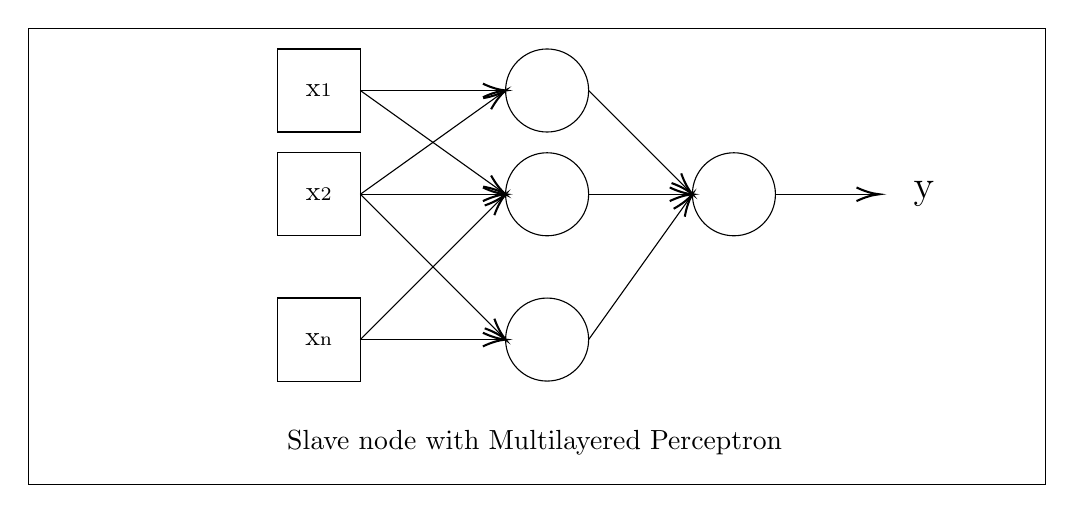
\begin{tikzpicture}[x=0.75pt,y=0.75pt,yscale=-1,xscale=1]
%uncomment if require: \path (0,300); %set diagram left start at 0, and has height of 300

%Shape: Rectangle [id:dp3356543770553979] 
\draw   (70,30) -- (560,30) -- (560,250) -- (70,250) -- cycle ;
%Shape: Square [id:dp5256435827897643] 
\draw   (190,40) -- (230,40) -- (230,80) -- (190,80) -- cycle ;
%Shape: Square [id:dp5270357160077517] 
\draw   (190,90) -- (230,90) -- (230,130) -- (190,130) -- cycle ;
%Shape: Square [id:dp06437153710385335] 
\draw   (190,160) -- (230,160) -- (230,200) -- (190,200) -- cycle ;
%Shape: Circle [id:dp6202571690827927] 
\draw   (300,60) .. controls (300,48.95) and (308.95,40) .. (320,40) .. controls (331.05,40) and (340,48.95) .. (340,60) .. controls (340,71.05) and (331.05,80) .. (320,80) .. controls (308.95,80) and (300,71.05) .. (300,60) -- cycle ;
%Shape: Circle [id:dp7260170908934287] 
\draw   (300,110) .. controls (300,98.95) and (308.95,90) .. (320,90) .. controls (331.05,90) and (340,98.95) .. (340,110) .. controls (340,121.05) and (331.05,130) .. (320,130) .. controls (308.95,130) and (300,121.05) .. (300,110) -- cycle ;
%Shape: Circle [id:dp9546670114782507] 
\draw   (300,180) .. controls (300,168.95) and (308.95,160) .. (320,160) .. controls (331.05,160) and (340,168.95) .. (340,180) .. controls (340,191.05) and (331.05,200) .. (320,200) .. controls (308.95,200) and (300,191.05) .. (300,180) -- cycle ;
%Shape: Circle [id:dp8873752821258001] 
\draw   (390,110) .. controls (390,98.95) and (398.95,90) .. (410,90) .. controls (421.05,90) and (430,98.95) .. (430,110) .. controls (430,121.05) and (421.05,130) .. (410,130) .. controls (398.95,130) and (390,121.05) .. (390,110) -- cycle ;
%Straight Lines [id:da6624191220110807] 
\draw    (230,60) -- (298,60) ;
\draw [shift={(300,60)}, rotate = 180] [color={rgb, 255:red, 0; green, 0; blue, 0 }  ][line width=0.75]    (10.93,-3.29) .. controls (6.95,-1.4) and (3.31,-0.3) .. (0,0) .. controls (3.31,0.3) and (6.95,1.4) .. (10.93,3.29)   ;
%Straight Lines [id:da0866384249373997] 
\draw    (230,110) -- (298,110) ;
\draw [shift={(300,110)}, rotate = 180] [color={rgb, 255:red, 0; green, 0; blue, 0 }  ][line width=0.75]    (10.93,-3.29) .. controls (6.95,-1.4) and (3.31,-0.3) .. (0,0) .. controls (3.31,0.3) and (6.95,1.4) .. (10.93,3.29)   ;
%Straight Lines [id:da13965027003077846] 
\draw    (230,180) -- (298,180) ;
\draw [shift={(300,180)}, rotate = 180] [color={rgb, 255:red, 0; green, 0; blue, 0 }  ][line width=0.75]    (10.93,-3.29) .. controls (6.95,-1.4) and (3.31,-0.3) .. (0,0) .. controls (3.31,0.3) and (6.95,1.4) .. (10.93,3.29)   ;
%Straight Lines [id:da7863905838920622] 
\draw    (230,60) -- (298.37,108.84) ;
\draw [shift={(300,110)}, rotate = 215.54] [color={rgb, 255:red, 0; green, 0; blue, 0 }  ][line width=0.75]    (10.93,-3.29) .. controls (6.95,-1.4) and (3.31,-0.3) .. (0,0) .. controls (3.31,0.3) and (6.95,1.4) .. (10.93,3.29)   ;
%Straight Lines [id:da16736595128940945] 
\draw    (230,110) -- (298.59,178.59) ;
\draw [shift={(300,180)}, rotate = 225] [color={rgb, 255:red, 0; green, 0; blue, 0 }  ][line width=0.75]    (10.93,-3.29) .. controls (6.95,-1.4) and (3.31,-0.3) .. (0,0) .. controls (3.31,0.3) and (6.95,1.4) .. (10.93,3.29)   ;
%Straight Lines [id:da837081391568496] 
\draw    (230,180) -- (298.59,111.41) ;
\draw [shift={(300,110)}, rotate = 495] [color={rgb, 255:red, 0; green, 0; blue, 0 }  ][line width=0.75]    (10.93,-3.29) .. controls (6.95,-1.4) and (3.31,-0.3) .. (0,0) .. controls (3.31,0.3) and (6.95,1.4) .. (10.93,3.29)   ;
%Straight Lines [id:da0751297016521475] 
\draw    (230,110) -- (298.37,61.16) ;
\draw [shift={(300,60)}, rotate = 504.46] [color={rgb, 255:red, 0; green, 0; blue, 0 }  ][line width=0.75]    (10.93,-3.29) .. controls (6.95,-1.4) and (3.31,-0.3) .. (0,0) .. controls (3.31,0.3) and (6.95,1.4) .. (10.93,3.29)   ;
%Straight Lines [id:da2549769311708434] 
\draw    (340,180) -- (388.84,111.63) ;
\draw [shift={(390,110)}, rotate = 485.54] [color={rgb, 255:red, 0; green, 0; blue, 0 }  ][line width=0.75]    (10.93,-3.29) .. controls (6.95,-1.4) and (3.31,-0.3) .. (0,0) .. controls (3.31,0.3) and (6.95,1.4) .. (10.93,3.29)   ;
%Straight Lines [id:da5966427506538203] 
\draw    (340,110) -- (388,110) ;
\draw [shift={(390,110)}, rotate = 180] [color={rgb, 255:red, 0; green, 0; blue, 0 }  ][line width=0.75]    (10.93,-3.29) .. controls (6.95,-1.4) and (3.31,-0.3) .. (0,0) .. controls (3.31,0.3) and (6.95,1.4) .. (10.93,3.29)   ;
%Straight Lines [id:da30294544760077824] 
\draw    (340,60) -- (388.59,108.59) ;
\draw [shift={(390,110)}, rotate = 225] [color={rgb, 255:red, 0; green, 0; blue, 0 }  ][line width=0.75]    (10.93,-3.29) .. controls (6.95,-1.4) and (3.31,-0.3) .. (0,0) .. controls (3.31,0.3) and (6.95,1.4) .. (10.93,3.29)   ;
%Straight Lines [id:da77593748506778] 
\draw    (430,110) -- (478,110) ;
\draw [shift={(480,110)}, rotate = 180] [color={rgb, 255:red, 0; green, 0; blue, 0 }  ][line width=0.75]    (10.93,-3.29) .. controls (6.95,-1.4) and (3.31,-0.3) .. (0,0) .. controls (3.31,0.3) and (6.95,1.4) .. (10.93,3.29)   ;

% Text Node
\draw (314,229.5) node   [align=left] {Slave node with Multilayered Perceptron};
% Text Node
\draw (210,60) node   [align=left] {x{\scriptsize 1}};
% Text Node
\draw (210,110) node   [align=left] {x{\scriptsize 2}};
% Text Node
\draw (210,180) node   [align=left] {x{\scriptsize n}};
% Text Node
\draw (501.5,110) node   [align=left] {{\Large y}};


\end{tikzpicture}
\end{figure}
%Step 2 end

\newpage
\item The chunks containing the data of the queries that were left unpredicted via the cluster are sent to the cluster in a round robin fashion. The method of sending the queries can be set to either round robin fashion or all at once. The 
%step 3

\tikzset{every picture/.style={line width=0.75pt}} %set default line width to 0.75pt        
\begin{figure}[!h]
\centering
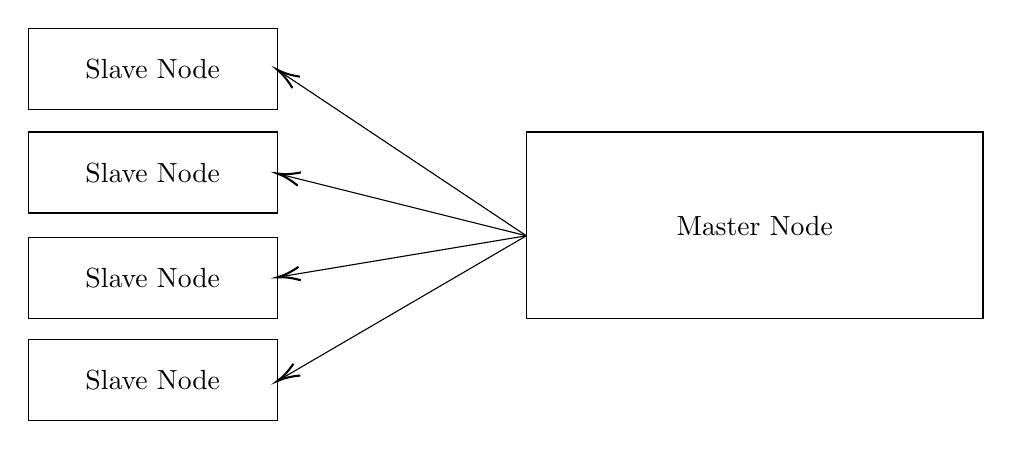
\begin{tikzpicture}[x=0.75pt,y=0.75pt,yscale=-1,xscale=1]
%uncomment if require: \path (0,300); %set diagram left start at 0, and has height of 300

%Shape: Rectangle [id:dp7056891731575645] 
\draw   (100,151) -- (220,151) -- (220,190) -- (100,190) -- cycle ;
%Shape: Rectangle [id:dp652502983568856] 
\draw   (100,200) -- (220,200) -- (220,239) -- (100,239) -- cycle ;
%Shape: Rectangle [id:dp1370792081503991] 
\draw   (100,50) -- (220,50) -- (220,89) -- (100,89) -- cycle ;
%Shape: Rectangle [id:dp3403063589466713] 
\draw   (100,100) -- (220,100) -- (220,139) -- (100,139) -- cycle ;
%Shape: Rectangle [id:dp05437739213565784] 
\draw   (340,100) -- (560,100) -- (560,190) -- (340,190) -- cycle ;
%Straight Lines [id:da17081303413935167] 
\draw    (340,150) -- (221.66,71.11) ;
\draw [shift={(220,70)}, rotate = 393.69] [color={rgb, 255:red, 0; green, 0; blue, 0 }  ][line width=0.75]    (10.93,-3.29) .. controls (6.95,-1.4) and (3.31,-0.3) .. (0,0) .. controls (3.31,0.3) and (6.95,1.4) .. (10.93,3.29)   ;
%Straight Lines [id:da6256697337377781] 
\draw    (340,150) -- (221.94,120.49) ;
\draw [shift={(220,120)}, rotate = 374.03999999999996] [color={rgb, 255:red, 0; green, 0; blue, 0 }  ][line width=0.75]    (10.93,-3.29) .. controls (6.95,-1.4) and (3.31,-0.3) .. (0,0) .. controls (3.31,0.3) and (6.95,1.4) .. (10.93,3.29)   ;
%Straight Lines [id:da3463514586442602] 
\draw    (340,150) -- (221.97,169.67) ;
\draw [shift={(220,170)}, rotate = 350.53999999999996] [color={rgb, 255:red, 0; green, 0; blue, 0 }  ][line width=0.75]    (10.93,-3.29) .. controls (6.95,-1.4) and (3.31,-0.3) .. (0,0) .. controls (3.31,0.3) and (6.95,1.4) .. (10.93,3.29)   ;
%Straight Lines [id:da6887749797140261] 
\draw    (340,150) -- (221.73,218.99) ;
\draw [shift={(220,220)}, rotate = 329.74] [color={rgb, 255:red, 0; green, 0; blue, 0 }  ][line width=0.75]    (10.93,-3.29) .. controls (6.95,-1.4) and (3.31,-0.3) .. (0,0) .. controls (3.31,0.3) and (6.95,1.4) .. (10.93,3.29)   ;

% Text Node
\draw (160,170.5) node   [align=left] {Slave Node};
% Text Node
\draw (160,219.5) node   [align=left] {Slave Node};
% Text Node
\draw (160,119.5) node   [align=left] {Slave Node};
% Text Node
\draw (160,69.5) node   [align=left] {Slave Node};
% Text Node
\draw (450,145) node   [align=left] {Master Node};


\end{tikzpicture}
\end{figure}

%step 3 end

\end{itemize}
\clearpage
\newpage
\section{Deploying to Cluster}
A cluster is a group of two or more servers connected to each other in such a way that they behave like a single server. Each machine in the cluster is called a node. Because each machine in the cluster runs the same services as other machines in the cluster, any machine can stand in for any other machine in the cluster. This becomes important when one machine goes down or must be taken out of service for a time. The remaining machines in the cluster can seamlessly take over the work of the downed machine, providing users with uninterrupted access to services and data.

\subsection{Benefits of Clustering}
\begin{itemize}
\item
Increased resource availability: If one Intelligence Server in a cluster fails, the other Intelligence Servers in the cluster can pick up the workload. This prevents the loss of valuable time and information if a server fails.
Strategic resource usage: You can distribute projects across nodes in whatever configuration you prefer. This reduces overhead because not all machines need to be running all projects, and allows you to use your resources flexibly.
\begin{itemize}
\item
Increased performance: Multiple machines provide greater processing power.
\item
Greater scalability: As your user base grows and report complexity increases, your resources can grow.
\item
Simplified management: Clustering simplifies the management of large or rapidly growing systems.
\item
Fail-over support ensures that a business intelligence system remains available for use if an application or hardware failure occurs. Clustering provides failover support in two ways:

Load redistribution: When a node fails, the work for which it is responsible is directed to another node or set of nodes.
Request recovery: When a node fails, the system attempts to reconnect MicroStrategy Web users with queued or processing requests to another node. Users must log in again to be authenticated on the new node. The user is prompted to resubmit job requests.

\end{itemize}
\end{itemize}
Load Balancing
Load balancing is a strategy aimed at achieving even distribution of user sessions across Intelligence Servers, so that no single machine is overwhelmed. This strategy is especially valuable when it is difficult to predict the number of requests a server will receive. MicroStrategy achieves four-tier load balancing by incorporating load balancers into the MicroStrategy Web and Web products.

Load is calculated as the number of user sessions connected to a node. The load balancers collect information on the number of user sessions each node is carrying. Using this information at the time a user logs in to a project, MicroStrategy Web connects them to the Intelligence Server node that is carrying the lightest session load. All requests by that user are routed to the node to which they are connected until the user disconnects from the MicroStrategy Web product.

Project Distribution and Project Fail over
When you set up several server machines in a cluster, you can distribute projects across those clustered machines or nodes in any configuration, in both Windows and Linux environments. All servers in a cluster do not need to be running all projects. Each node in the cluster can host a different set of projects, which means only a subset of projects need to be loaded on a specific Intelligence Server machine. This feature provides you with flexibility in using your resources, and it provides better scalability and performance because of less overhead on each Intelligence Server machine.

Distributing projects across nodes also provides project fail-over support. For example, one server is hosting project A and another server is hosting projects B and C. If the first server fails, the other server can host all three projects to ensure project availability.

Project creation, duplication, and deletion in a three-tier, or server, connection are automatically broadcast to all nodes during run-time to ensure synchronization across the cluster.

Work Fencing
User fences and workload fences allow you to reserve nodes of a cluster for either users or a project subscriptions. 

\newpage
\section{Future Scope}

\newpage
\section{Tables}
{
\clearpage
\thispagestyle{empty}
\begin{landscape}
\centering
\begin{table}[]
\centering
\begin{tabular}{|l|l|}
\hline
Column Name                & Description                                                               \\ \hline
Pregnancies                & Number of times pregnant.                                                 \\ \hline
Glucose                    & Plasma glucose concentration a 2 hours in an oral glucose tolerance test. \\ \hline
Blood Pressure             & Diastolic blood pressure (mm Hg)                                          \\ \hline
Skin Thickness             & Triceps skin fold thickness (mm)                                          \\ \hline
Insulin                    & 2-Hour serum insulin (muU/ml)                                            \\ \hline
Body Mass Index            & Body mass index (weight in kg/(height in m)\textasciicircum{}2)           \\ \hline
Diabetes Pedigree Function & Diabetes pedigree function                                                \\ \hline
Age                        & Age (years)                                                               \\ \hline
Outcome                    & Class variable (0 or 1) 268 of 768 are 1, the others are 0                \\ \hline
\end{tabular}
\end{table}
\captionof{table}{Pima Indians dataset header.}
\label{table:1}
\end{landscape}
\clearpage
}


{
\clearpage
\thispagestyle{empty}
\begin{landscape}
\centering
\begin{table}[]
\begin{tabular}{|c|c|c|c|}
\hline
Algorithm              & Additional Parameters                              & Train Set Accuracy & Test Set Accuracy \\ \hline
K Nearest Neighbour    & -                                                  & 0.79               & 0.78              \\ \hline
Logistic Regression    & C = 1                                              & 0.781              & 0.771             \\ \hline
Logistic Regression    & C = 0.01                                           & 0.700              & 0.703             \\ \hline
Logistic Regression    & C = 100                                            & 0.785              & 0.766             \\ \hline
Decision Tree          & -                                                  & 1.00               & 0.714             \\ \hline
Decision Tree          & Max Depth = 3                                      & 0.773              & 0.740             \\ \hline
Random Forest          & Estimators = 100                                   & 1.000              & 0.786             \\ \hline
Random Forest          & Estimators = 100; Max Depth = 3                    & 0.800              & 0.755             \\ \hline
Gradient Boosting      & -                                                  & 0.917              & 0.792             \\ \hline
Gradient Boosting      & Max Depth = 1                                      & 0.804              & 0.781             \\ \hline
Gradient Boosting      & Learning Rate = 0.01                               & 0.802              & 0.776             \\ \hline
Support Vector Machine & -                                                  & 1.00               & 0.65              \\ \hline
Support Vector Machine & Train and Test set scaled using MinMaxScaler       & 0.77               & 0.77              \\ \hline
Support Vector Machine & C = 1000                                           & 0.790              & 0.797             \\ \hline
MLP Classifier         & Random State = 42                                  & 0.73               & 0.72              \\ \hline
MLP Classifier         & Random State = 0                                   & 0.823              & 0.802             \\ \hline
MLP Classifier         & Max Iterations = 1000                              & 0.908              & 0.792             \\ \hline
MLP Classifier         & Max Iterations = 1000; Alpha = 1; Random State = 0 & 0.806              & 0.797             \\ \hline
\end{tabular}
\end{table}
\captionof{table}{Test and Train accuracy's using various machine learning algorithms with various parameters.}
\label{table:2}
\end{landscape}
\clearpage
}

\newpage
\section{Appendices}
\subsection{K Nearest Neighbours}
\begin{lstlisting}
class sklearn.neighbors.KNeighborsClassifier(n_neighbors=5, weights='uniform', algorithm='auto', leaf_size=30, p=2, metric='minkowski', metric_params=None, n_jobs=None, **kwargs)
\end{lstlisting}

\subsubsection{Logistic Regression}
\begin{lstlisting}
class sklearn.linear_model.LogisticRegression(penalty='l2', dual=False, tol=0.0001, C=1.0, fit_intercept=True, intercept_scaling=1, class_weight=None, random_state=None, solver='lbfgs', max_iter=100, multi_class='auto', verbose=0, warm_start=False, n_jobs=None, l1_ratio=None)
\end{lstlisting}

\subsubsection{Decision Tree}
\begin{lstlisting}
class sklearn.tree.DecisionTreeClassifier(criterion='gini', splitter='best', max_depth=None, min_samples_split=2, min_samples_leaf=1, min_weight_fraction_leaf=0.0, max_features=None, random_state=None, max_leaf_nodes=None, min_impurity_decrease=0.0, min_impurity_split=None, class_weight=None, presort='deprecated', ccp_alpha=0.0)
\end{lstlisting}

\subsubsection{Random Forest Classifier}
\begin{lstlisting}
class sklearn.ensemble.RandomForestClassifier(n_estimators=100, criterion='gini', max_depth=None, min_samples_split=2, min_samples_leaf=1, min_weight_fraction_leaf=0.0, max_features='auto', max_leaf_nodes=None, min_impurity_decrease=0.0, min_impurity_split=None, bootstrap=True, oob_score=False, n_jobs=None, random_state=None, verbose=0, warm_start=False, class_weight=None, ccp_alpha=0.0, max_samples=None)
\end{lstlisting}

\subsubsection{Gradient Boosting}
\begin{lstlisting}
class sklearn.ensemble.GradientBoostingClassifier(loss='deviance', learning_rate=0.1, n_estimators=100, subsample=1.0, criterion='friedman_mse', min_samples_split=2, min_samples_leaf=1, min_weight_fraction_leaf=0.0, max_depth=3, min_impurity_decrease=0.0, min_impurity_split=None, init=None, random_state=None, max_features=None, verbose=0, max_leaf_nodes=None, warm_start=False, presort='deprecated', validation_fraction=0.1, n_iter_no_change=None, tol=0.0001, ccp_alpha=0.0)
\end{lstlisting}

\subsubsection{Multi Layered Perceptron}
\begin{lstlisting}
class sklearn.neural_network.MLPClassifier(hidden_layer_sizes=(100, ), activation='relu', solver='adam', alpha=0.0001, batch_size='auto', learning_rate='constant', learning_rate_init=0.001, power_t=0.5, max_iter=200, shuffle=True, random_state=None, tol=0.0001, verbose=False, warm_start=False, momentum=0.9, nesterovs_momentum=True, early_stopping=False, validation_fraction=0.1, beta_1=0.9, beta_2=0.999, epsilon=1e-08, n_iter_no_change=10, max_fun=15000)
\end{lstlisting}

\subsection{SVM}
\begin{lstlisting}
class sklearn.svm.SVC(C=1.0, kernel='rbf', degree=3, gamma='scale', coef0=0.0, shrinking=True, probability=False, tol=0.001, cache_size=200, class_weight=None, verbose=False, max_iter=-1, decision_function_shape='ovr', break_ties=False, random_state=None)
\end{lstlisting}

\clearpage
%include for many images
\maxdeadcycles=1000


\begin{figure}[ht]
\centering
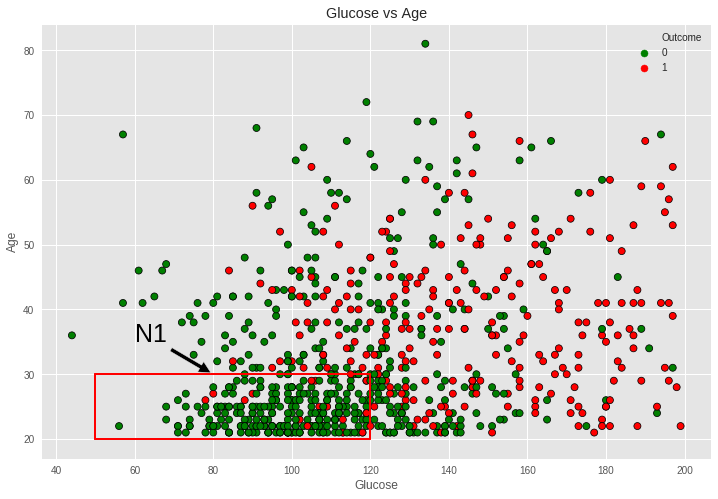
\includegraphics[width=1\textwidth]{download(1).png}
\caption{Master Node reading data from the SQL Database.}
\end{figure}

\begin{figure}[ht]
\centering
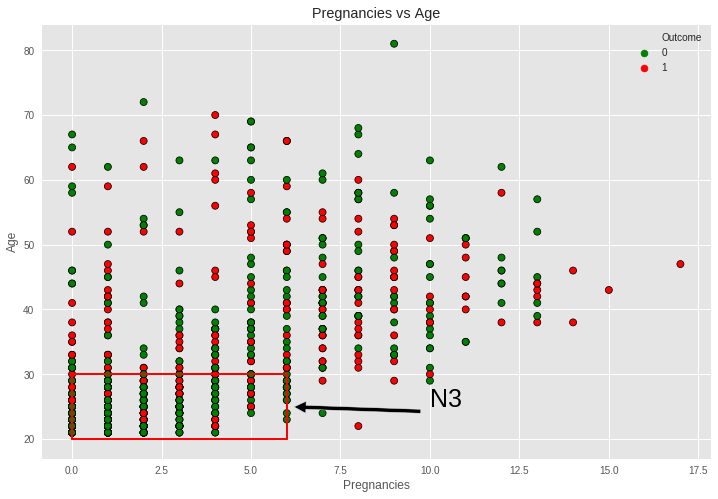
\includegraphics[width=1\textwidth]{download(2).png}
\caption{Master Node reading data from the SQL Database.}
\end{figure}

\begin{figure}[ht]
\centering
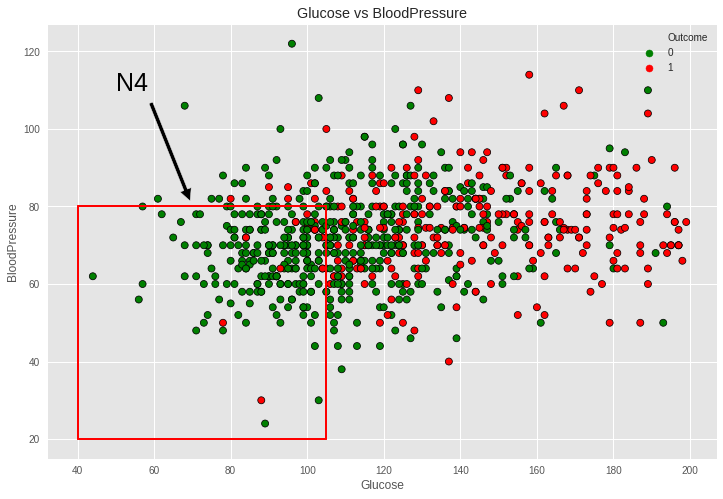
\includegraphics[width=1\textwidth]{download(3).png}
\caption{Master Node reading data from the SQL Database.}
\end{figure}

\begin{figure}[ht]
\centering
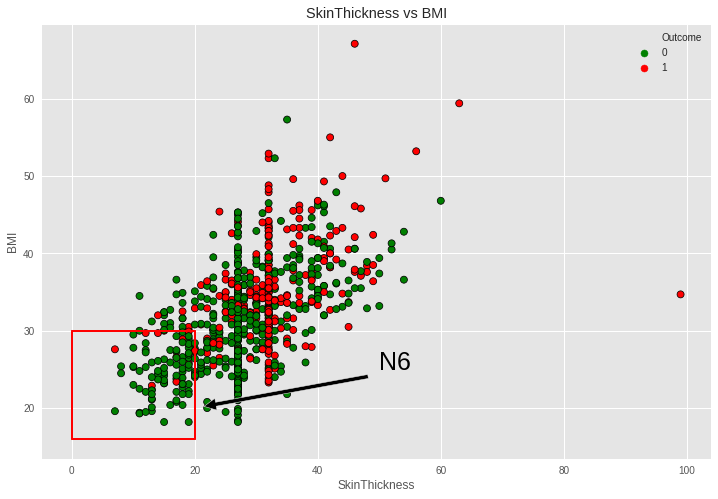
\includegraphics[width=1\textwidth]{download(4).png}
\caption{Master Node reading data from the SQL Database.}
\end{figure}

\begin{figure}[ht]
\centering
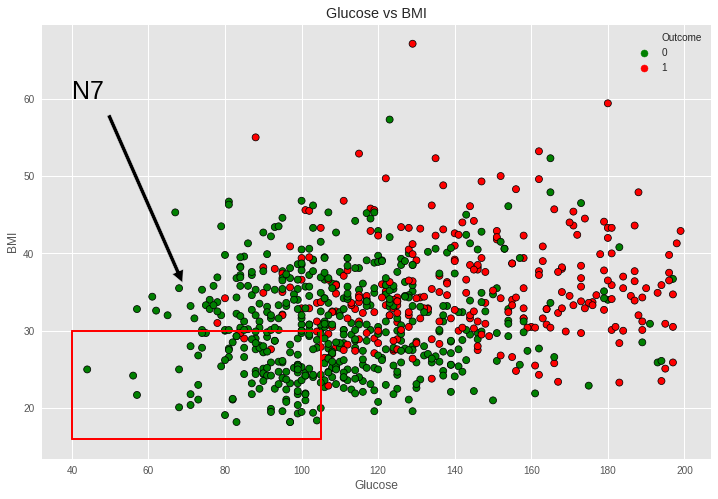
\includegraphics[width=1\textwidth]{download(5).png}
\caption{Master Node reading data from the SQL Database.}
\end{figure}

\begin{figure}[ht]
\centering
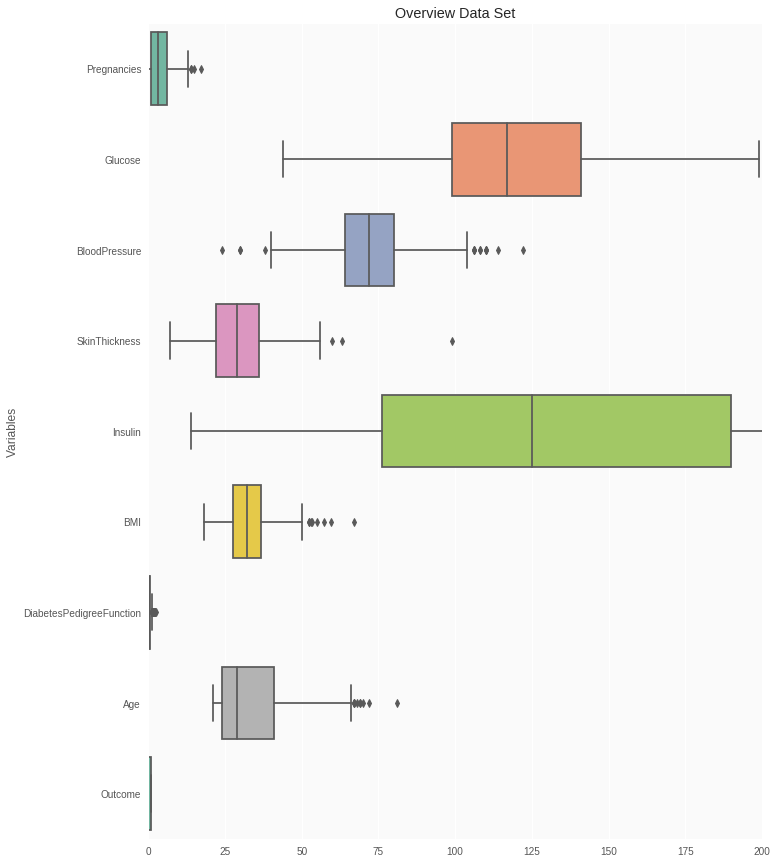
\includegraphics[width=1\textwidth]{download.png}
\caption{Master Node reading data from the SQL Database.}
\end{figure}

\begin{figure}[ht]
\centering
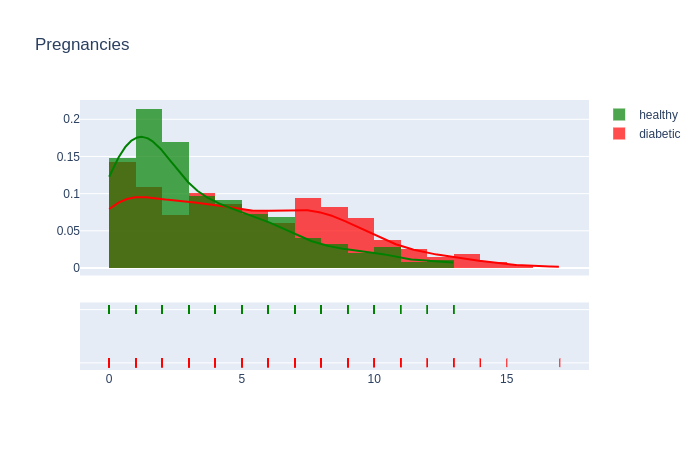
\includegraphics[width=1\textwidth]{newplot(10).png}
\caption{Master Node reading data from the SQL Database.}
\end{figure}

\begin{figure}[ht]
\centering
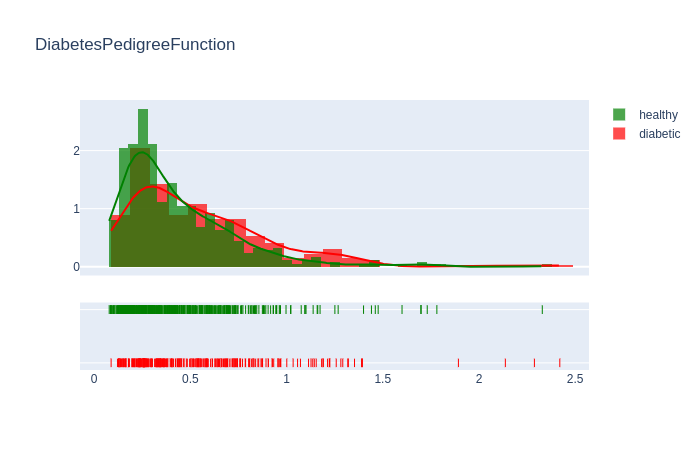
\includegraphics[width=1\textwidth]{newplot(11).png}
\caption{Master Node reading data from the SQL Database.}
\end{figure}

\begin{figure}[ht]
\centering
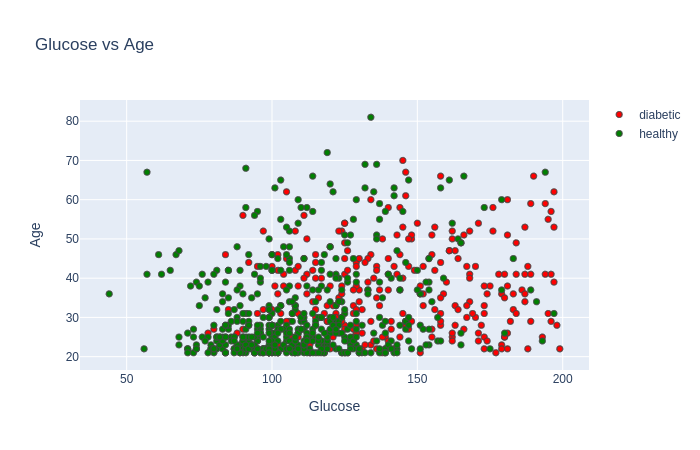
\includegraphics[width=1\textwidth]{newplot(12).png}
\caption{Master Node reading data from the SQL Database.}
\end{figure}

\begin{figure}[ht]
\centering
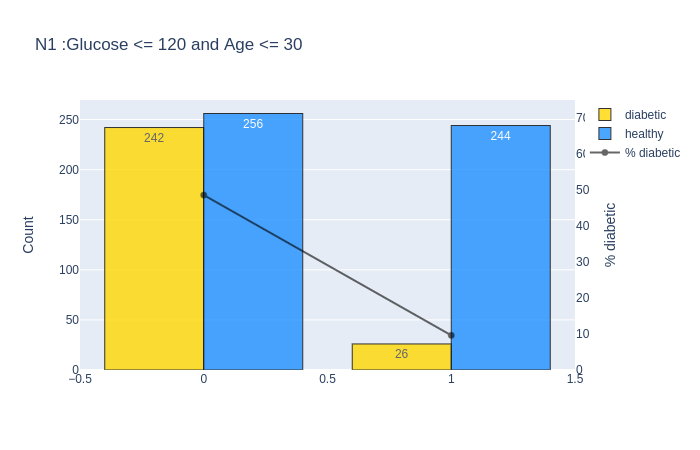
\includegraphics[width=1\textwidth]{newplot(13).png}
\caption{Master Node reading data from the SQL Database.}
\end{figure}

\begin{figure}[ht]
\centering
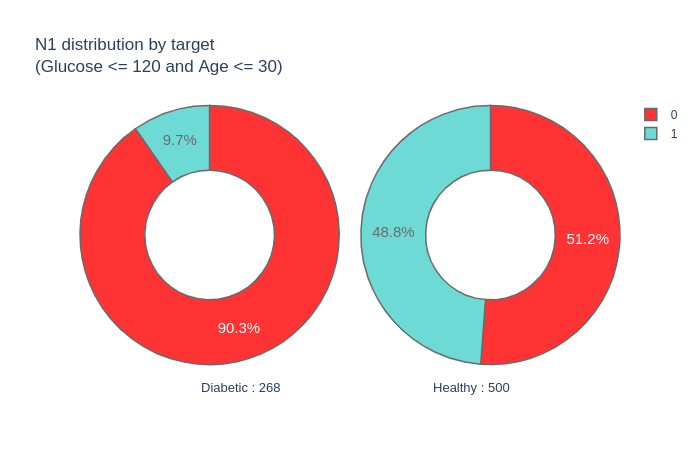
\includegraphics[width=1\textwidth]{newplot(14).png}
\caption{Master Node reading data from the SQL Database.}
\end{figure}

\begin{figure}[ht]
\centering
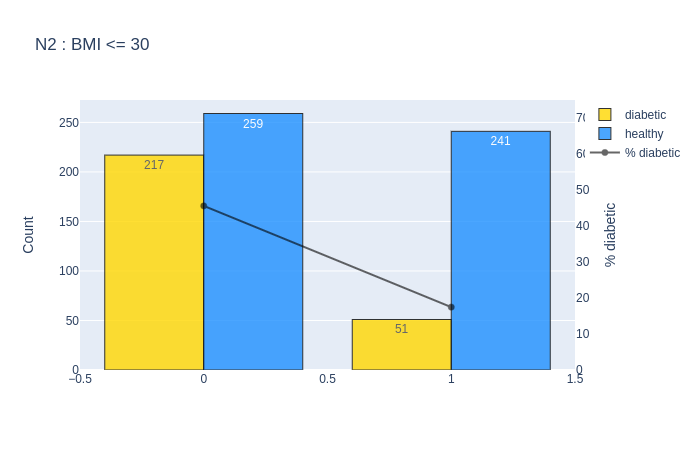
\includegraphics[width=1\textwidth]{newplot(15).png}
\caption{Master Node reading data from the SQL Database.}
\end{figure}

\begin{figure}[ht]
\centering
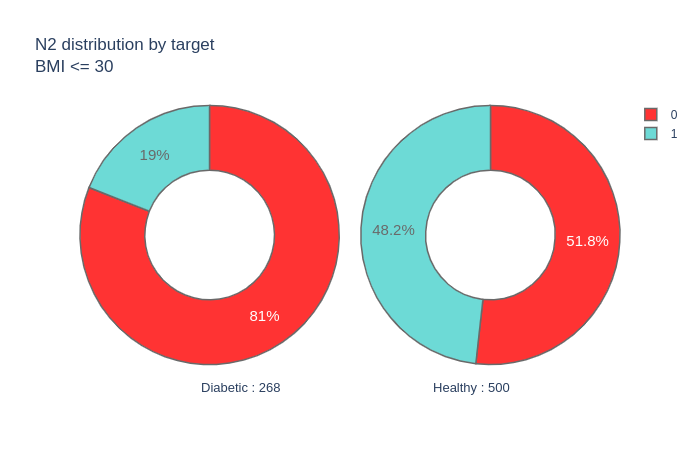
\includegraphics[width=1\textwidth]{newplot(16).png}
\caption{Master Node reading data from the SQL Database.}
\end{figure}

\begin{figure}[ht]
\centering
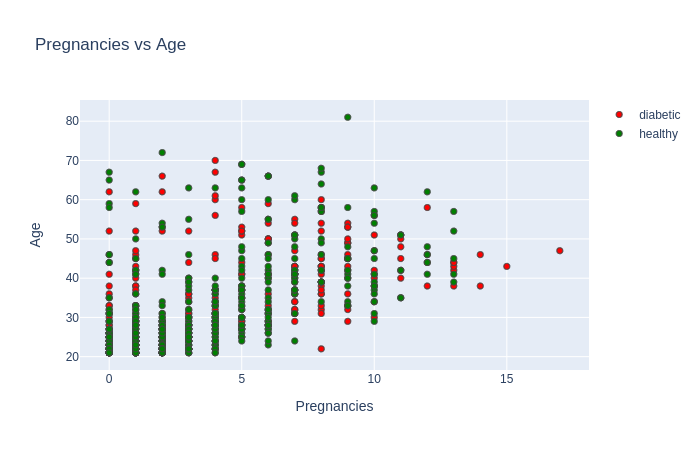
\includegraphics[width=1\textwidth]{newplot(17).png}
\caption{Master Node reading data from the SQL Database.}
\end{figure}

\begin{figure}[ht]
\centering
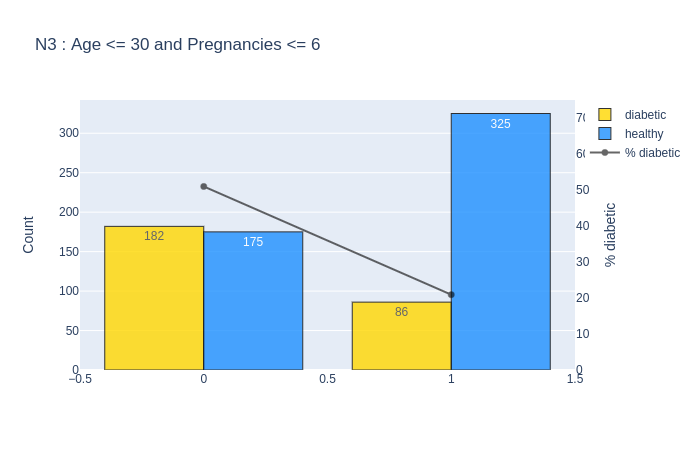
\includegraphics[width=1\textwidth]{newplot(18).png}
\caption{Master Node reading data from the SQL Database.}
\end{figure}

\begin{figure}[ht]
\centering
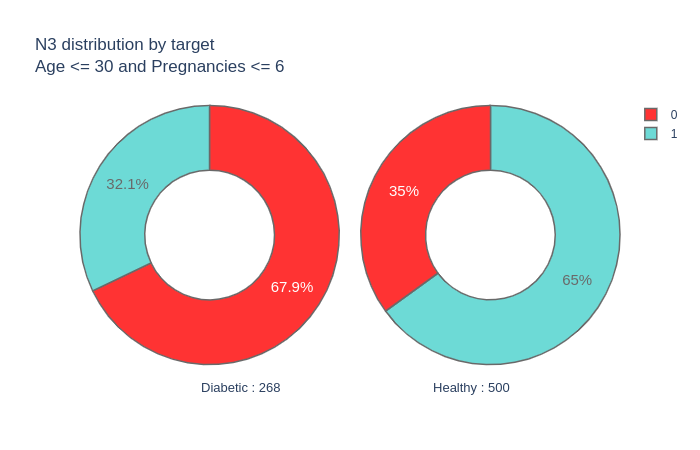
\includegraphics[width=1\textwidth]{newplot(19).png}
\caption{Master Node reading data from the SQL Database.}
\end{figure}

\begin{figure}[ht]
\centering
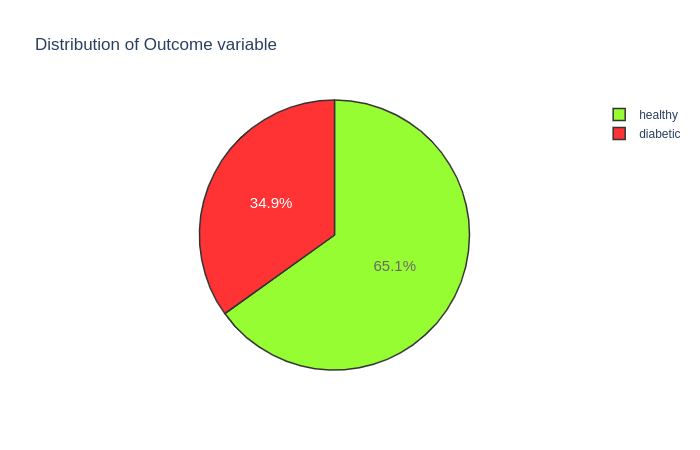
\includegraphics[width=1\textwidth]{newplot(1).png}
\caption{Master Node reading data from the SQL Database.}
\end{figure}

\begin{figure}[ht]
\centering
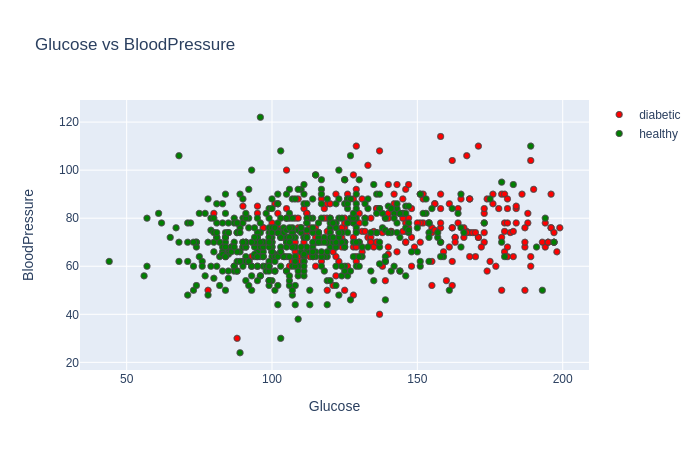
\includegraphics[width=1\textwidth]{newplot(20).png}
\caption{Master Node reading data from the SQL Database.}
\end{figure}

\begin{figure}[ht]
\centering
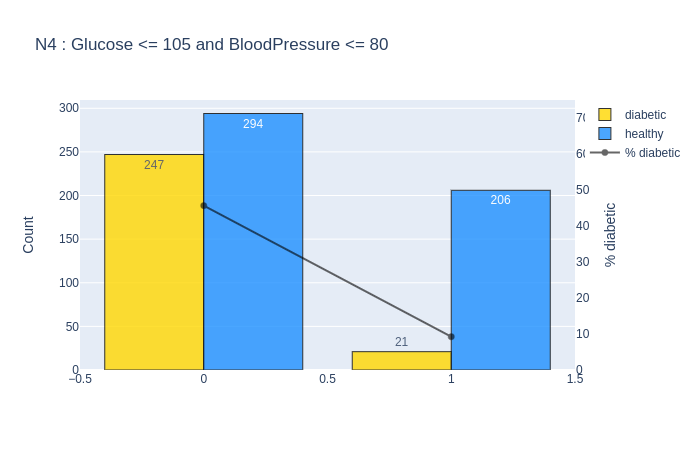
\includegraphics[width=1\textwidth]{newplot(21).png}
\caption{Master Node reading data from the SQL Database.}
\end{figure}

\begin{figure}[ht]
\centering
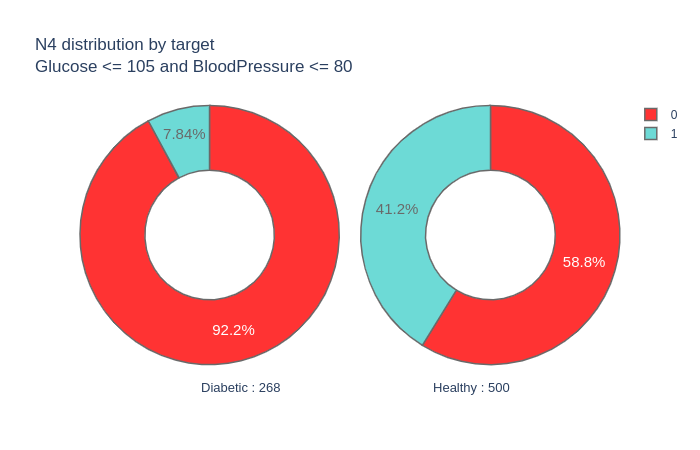
\includegraphics[width=1\textwidth]{newplot(22).png}
\caption{Master Node reading data from the SQL Database.}
\end{figure}

\begin{figure}[ht]
\centering
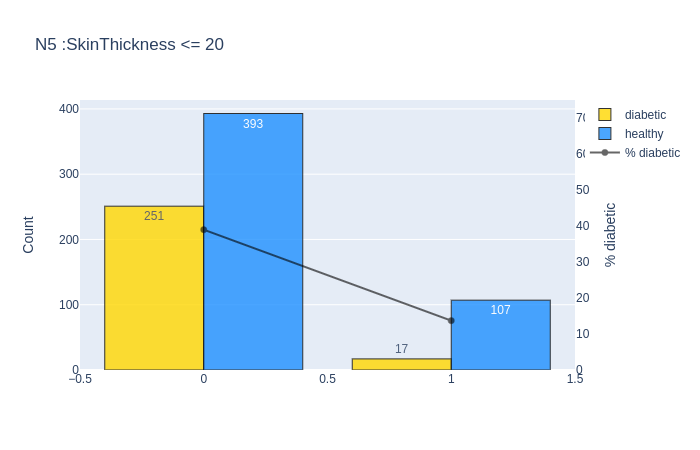
\includegraphics[width=1\textwidth]{newplot(23).png}
\caption{Master Node reading data from the SQL Database.}
\end{figure}

\begin{figure}[ht]
\centering
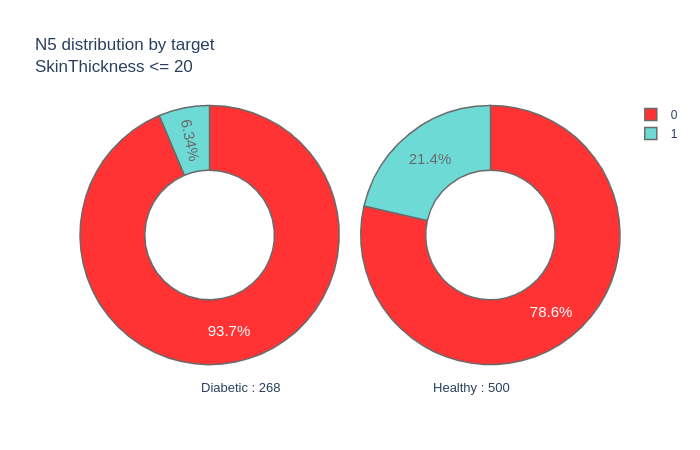
\includegraphics[width=1\textwidth]{newplot(24).png}
\caption{Master Node reading data from the SQL Database.}
\end{figure}

\begin{figure}[ht]
\centering
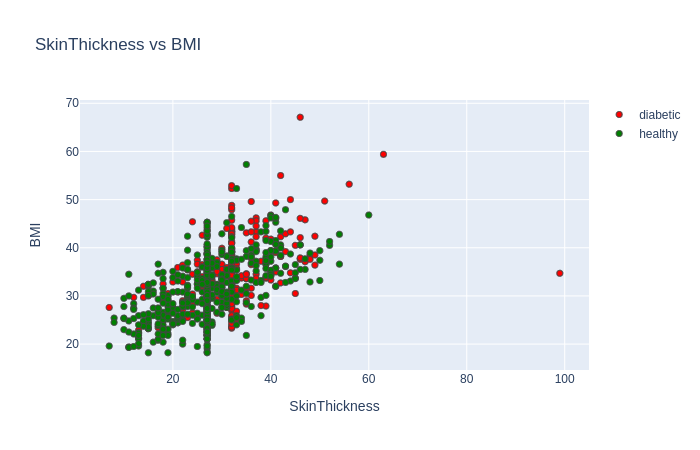
\includegraphics[width=1\textwidth]{newplot(25).png}
\caption{Master Node reading data from the SQL Database.}
\end{figure}

\begin{figure}[ht]
\centering
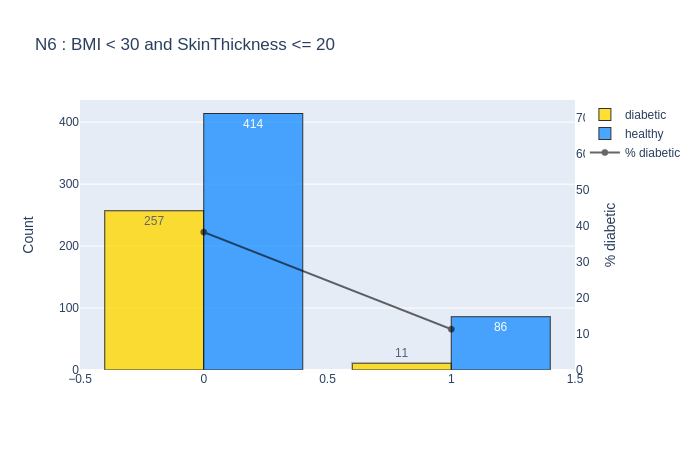
\includegraphics[width=1\textwidth]{newplot(26).png}
\caption{N6 Distribution by target.}
\end{figure}

\begin{figure}[ht]
\centering
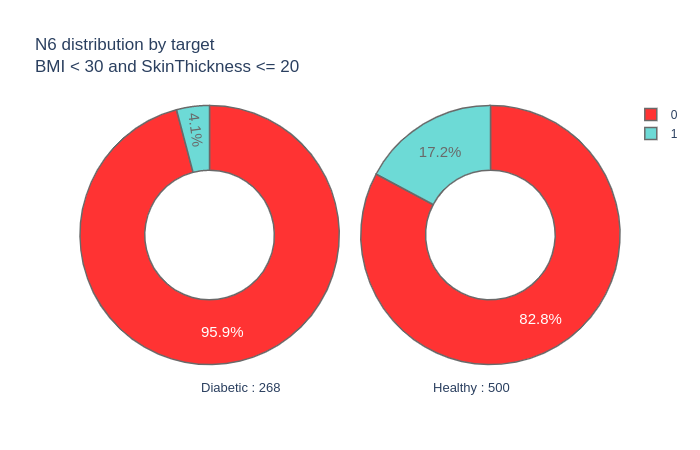
\includegraphics[width=1\textwidth]{newplot(27).png}
\caption{Glucose v/s BMI}
\end{figure}

\begin{figure}[ht]
\centering
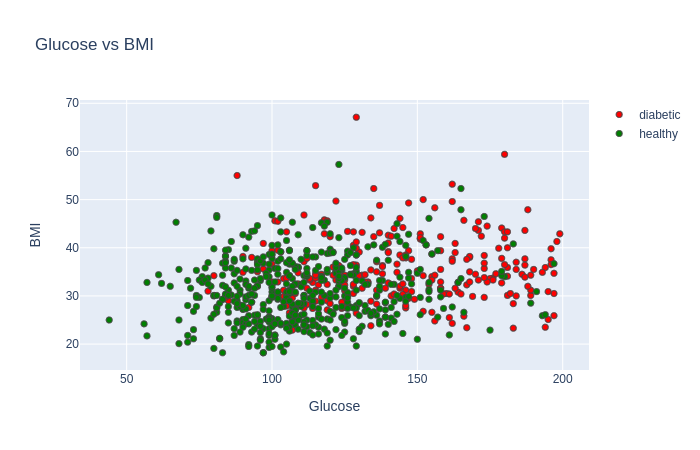
\includegraphics[width=1\textwidth]{newplot(28).png}
\caption{N7}
\end{figure}

\begin{figure}[ht]
\centering
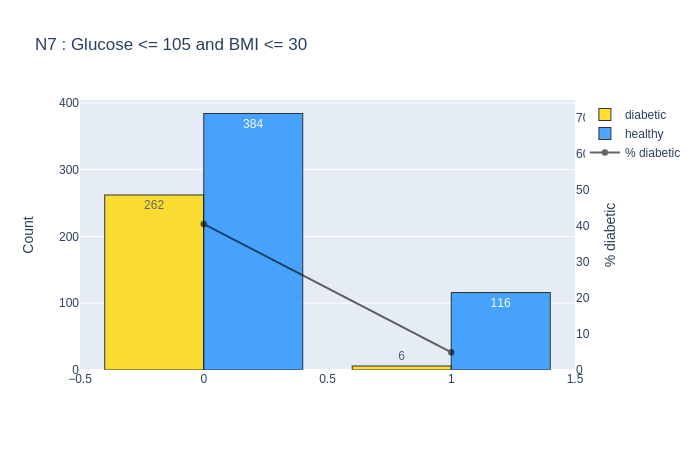
\includegraphics[width=1\textwidth]{newplot(29).png}
\caption{Missing values in count and percentage.}
\end{figure}

\begin{figure}[ht]
\centering
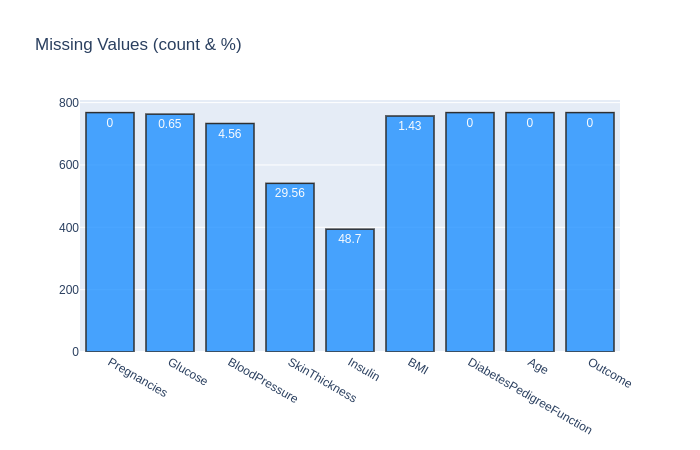
\includegraphics[width=1\textwidth]{newplot(2).png}
\caption{N7 distribution by target.}
\end{figure}

\begin{figure}[ht]
\centering
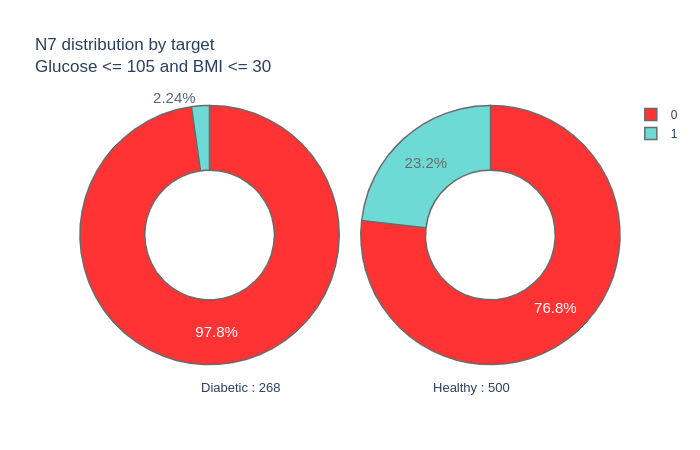
\includegraphics[width=1\textwidth]{newplot(30).png}
\caption{N7.}
\end{figure}


\begin{figure}[ht]
\centering
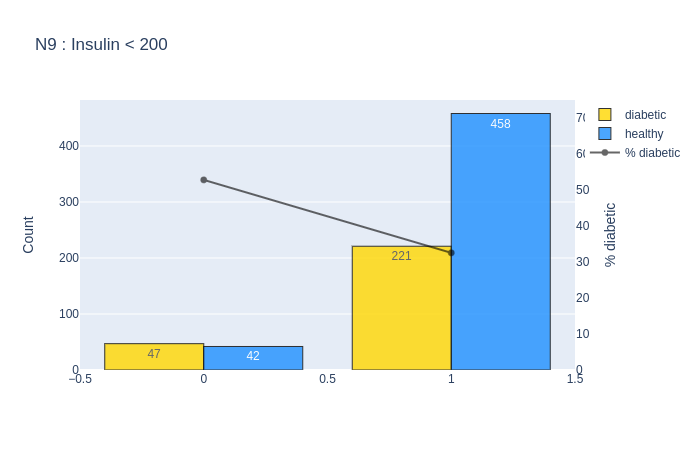
\includegraphics[width=1\textwidth]{newplot(32).png}
\caption{N9 distribution by target.}
\end{figure}

\begin{figure}[ht]
\centering
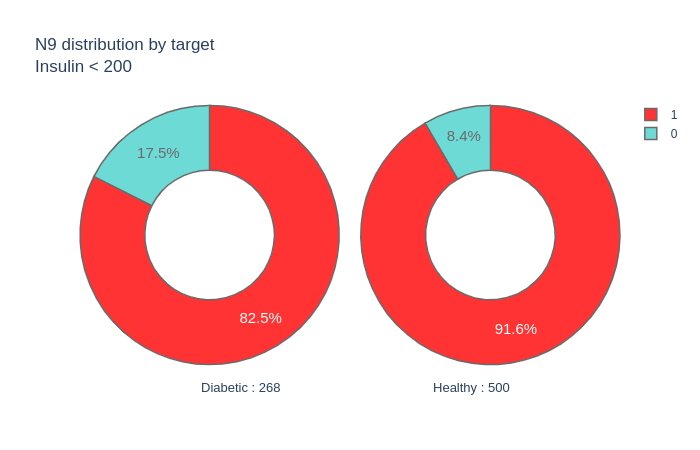
\includegraphics[width=1\textwidth]{newplot(33).png}
\caption{N10 distribution for diabetic and healthy people bp<80.}
\end{figure}

\begin{figure}[ht]
\centering
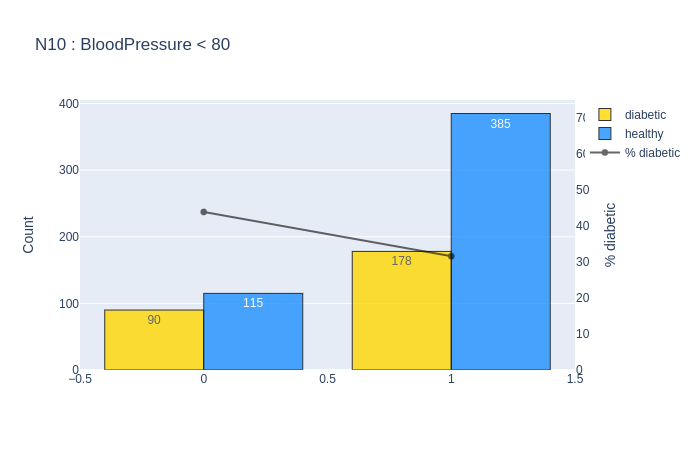
\includegraphics[width=1\textwidth]{newplot(34).png}
\caption{N10 distribution for diabetic and healthy people.}
\end{figure}

\begin{figure}[ht]
\centering
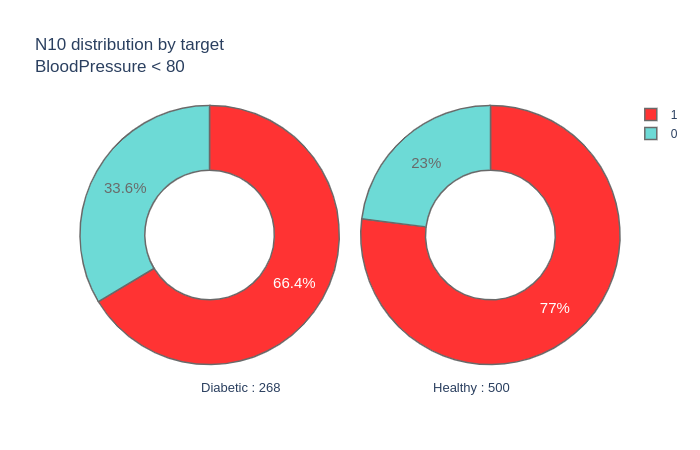
\includegraphics[width=1\textwidth]{newplot(35).png}
\caption{Pregnancies distribution for diabetic and healthy people.}
\end{figure}

\begin{figure}[ht]
\centering
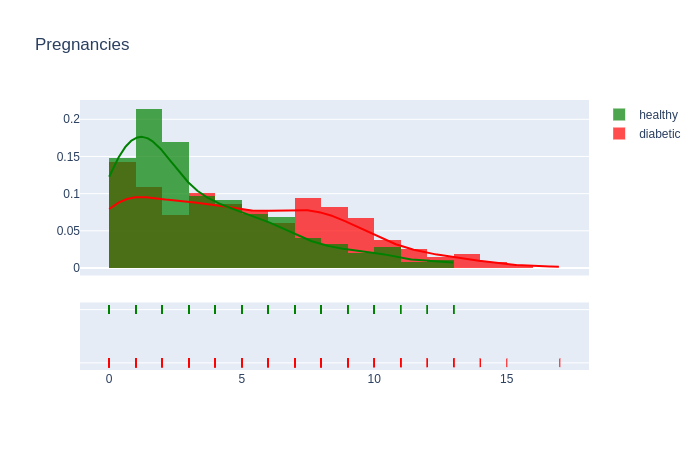
\includegraphics[width=1\textwidth]{newplot(36).png}
\caption{N11 feature obtained with patients > 0 and < 4.}
\end{figure}

\begin{figure}[ht]
\centering
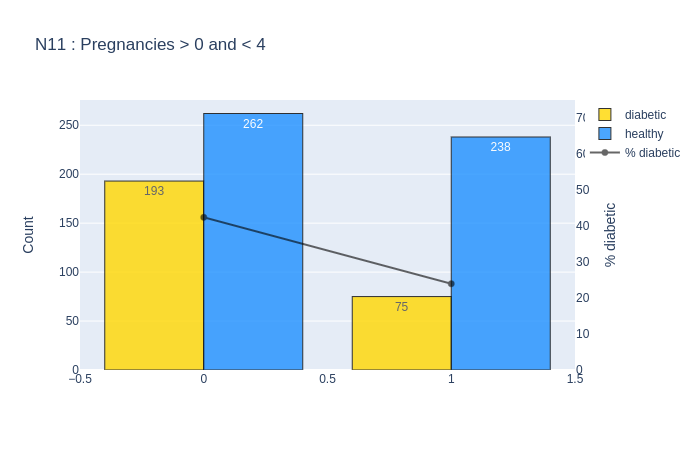
\includegraphics[width=1\textwidth]{newplot(37).png}
\caption{N11 distribution via target labels.}
\end{figure}

\begin{figure}[ht]
\centering
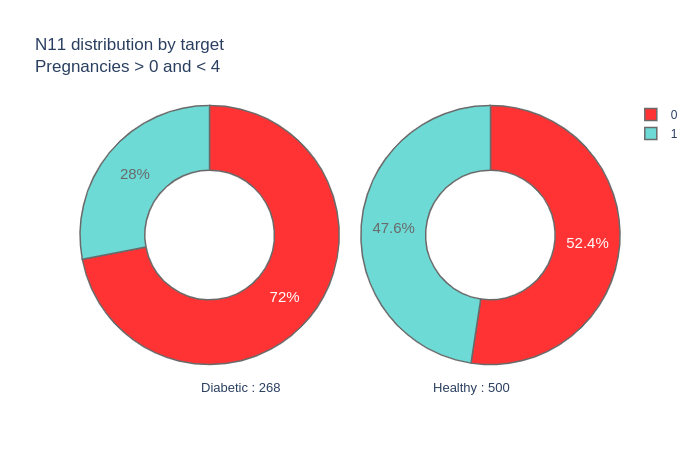
\includegraphics[width=1\textwidth]{newplot(38).png}
\caption{N0 Distribution.}
\end{figure}

\begin{figure}[ht]
\centering
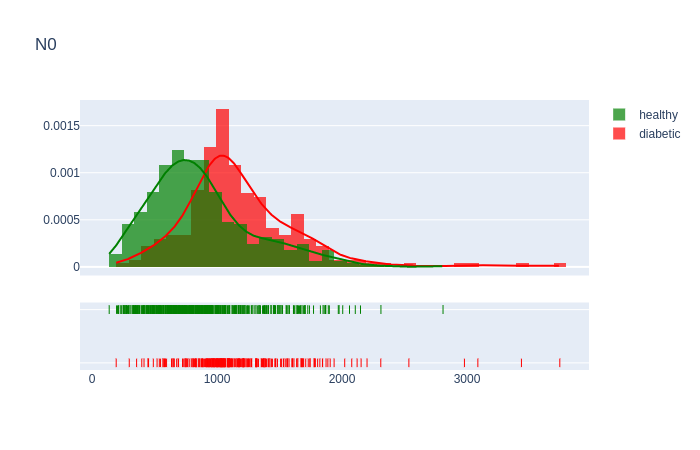
\includegraphics[width=1\textwidth]{newplot(39).png}
\caption{Correlation plot of raw dataset.}
\end{figure}

\begin{figure}[ht]
\centering
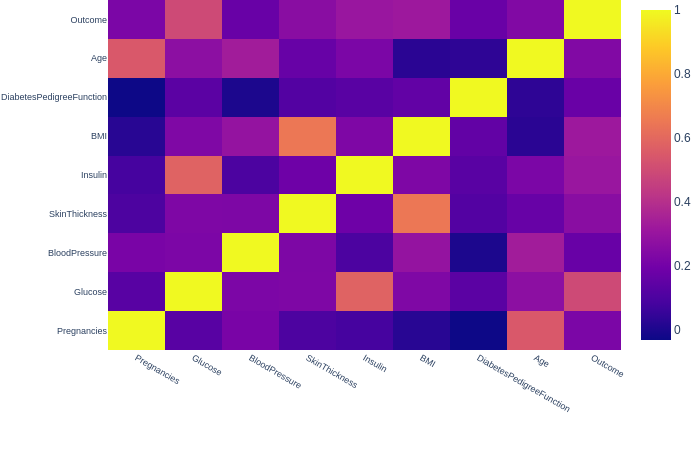
\includegraphics[width=1\textwidth]{newplot(3).png}
\caption{N15 where N0 is less than 1034.}
\end{figure}

\begin{figure}[ht]
\centering
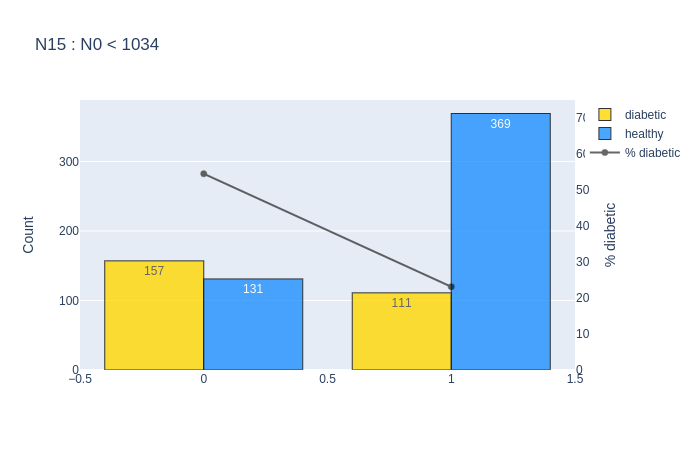
\includegraphics[width=1\textwidth]{newplot(40).png}
\caption{N15 distribution by target labels.}
\end{figure}

\begin{figure}[ht]
\centering
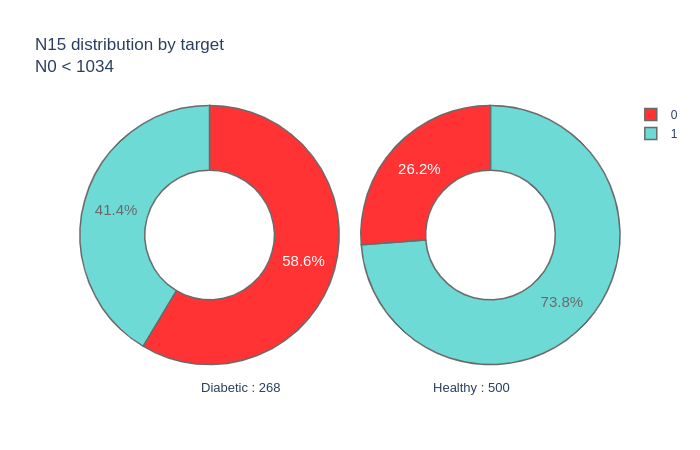
\includegraphics[width=1\textwidth]{newplot(41).png}
\caption{Correlation plot with newly added features.}
\end{figure}

\begin{figure}[ht]
\centering
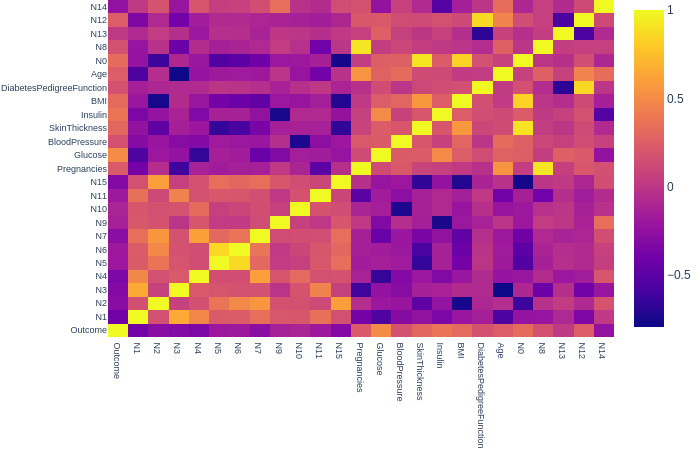
\includegraphics[width=1\textwidth]{newplot(42).png}
\caption{Model Performance report measured with 5 fold iterations.}
\end{figure}

\begin{figure}[ht]
\centering
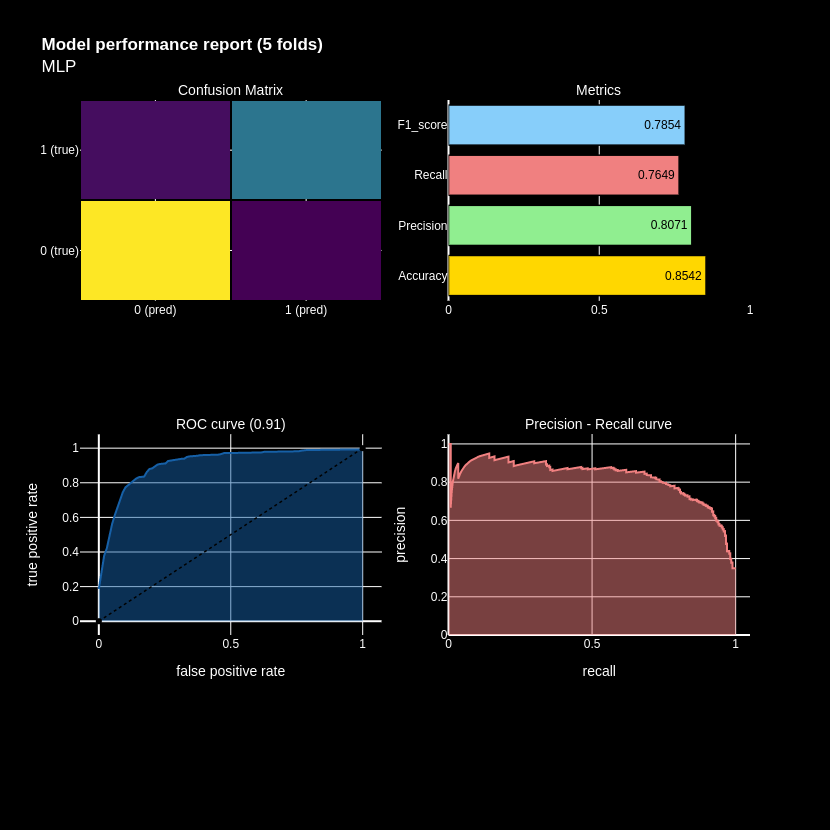
\includegraphics[width=1\textwidth]{newplot(43).png}
\caption{5 Fold Cross Validation score for the MLP Classifier.}
\end{figure}

\begin{figure}[ht]
\centering
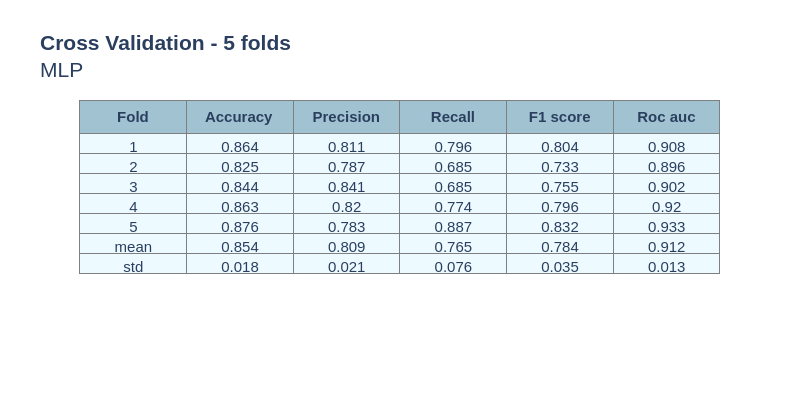
\includegraphics[width=1\textwidth]{newplot(44).png}
\caption{Insulin distribution for diabetic and healthy people.}
\end{figure}

\begin{figure}[ht]
\centering
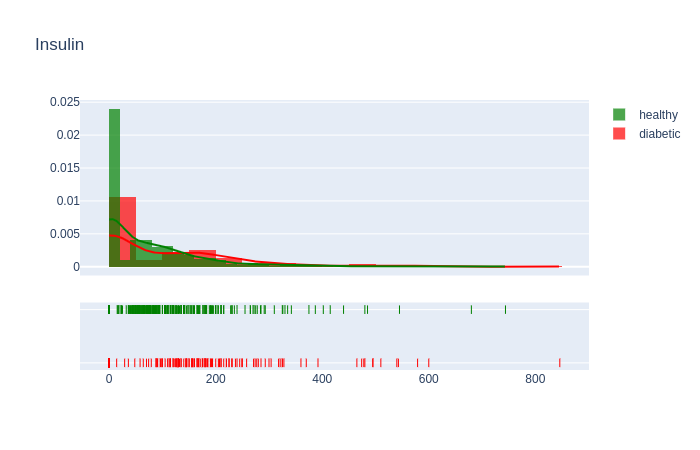
\includegraphics[width=1\textwidth]{newplot(4).png}
\caption{Glucose distribution for diabetic and healthy people.}
\end{figure}

\begin{figure}[ht]
\centering
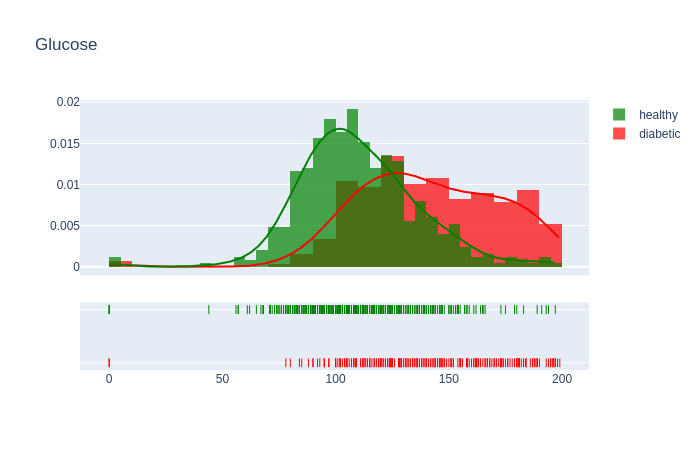
\includegraphics[width=1\textwidth]{newplot(5).png}
\caption{Master Node reading data from the SQL Database.}
\end{figure}

\begin{figure}[ht]
\centering
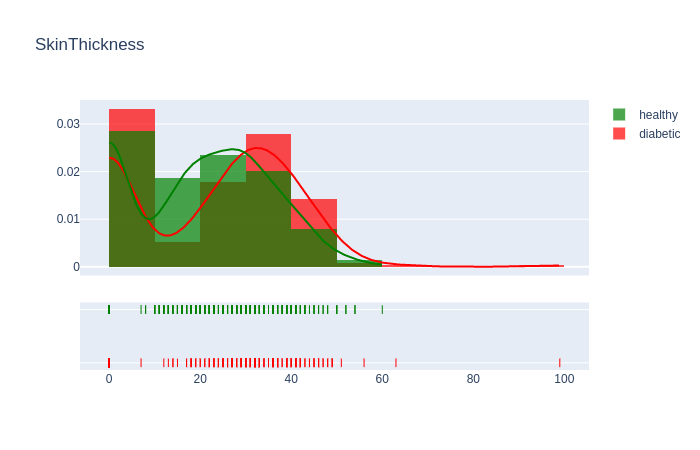
\includegraphics[width=1\textwidth]{newplot(6).png}
\caption{Skin Thickness distribution for diabetic and healthy people.}
\end{figure}

\begin{figure}[ht]
\centering
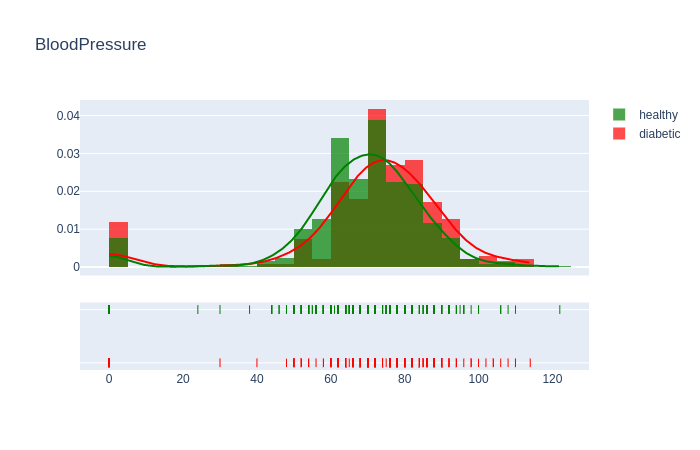
\includegraphics[width=1\textwidth]{newplot(7).png}
\caption{Blood pressure distribution for diabetic and healthy people.}
\end{figure}

\begin{figure}[ht]
\centering
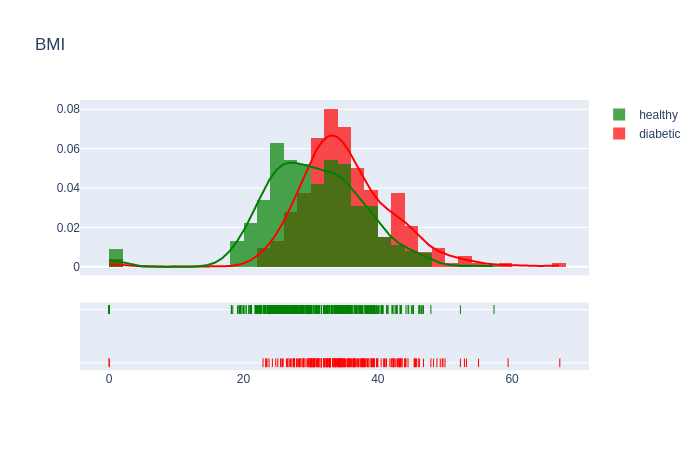
\includegraphics[width=1\textwidth]{newplot(8).png}
\caption{BMI distribution for diabetic and healthy people.}
\end{figure}

\begin{figure}[ht]
\centering
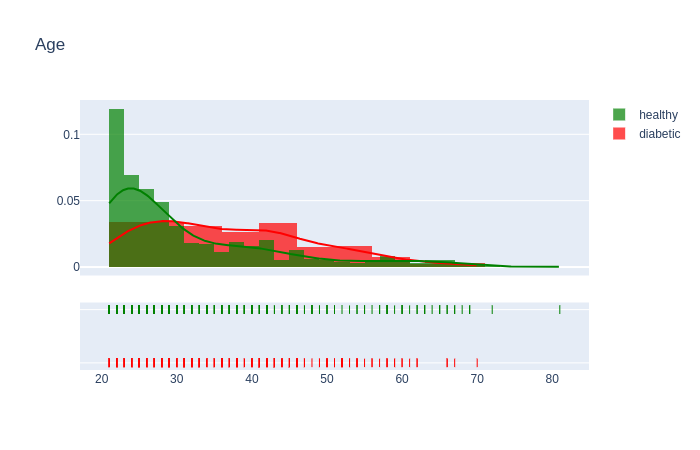
\includegraphics[width=1\textwidth]{newplot(9).png}
\caption{Age distribution for diabetic and healthy people.}
\end{figure}

\begin{figure}[ht]
\centering
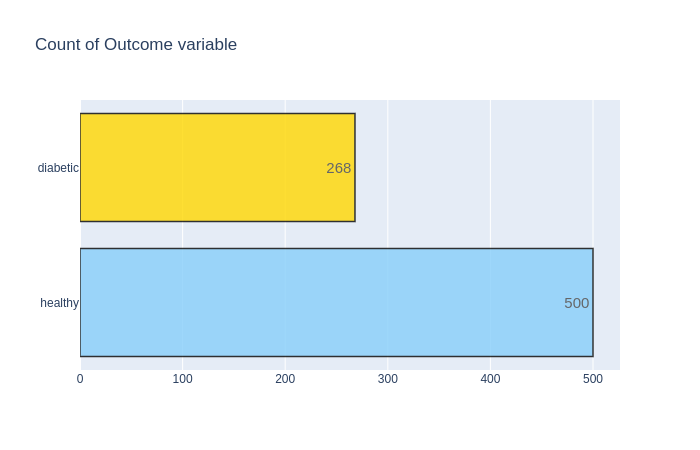
\includegraphics[width=1\textwidth]{newplot.png}
\caption{Count of Outcome Variable.}
\end{figure}
\clearpage
\newpage
\section{Student Profile}

\clearpage
\newpage
\section{Conclusion}
%https://www.scott-clark.com/2018/10/01/types-of-information-systems-used-in-healthcare-facilities/
%https://doc-archives.microstrategy.com/producthelp/10.11/SystemAdmin/WebHelp/Lang_1033/Content/Benefits_of_clustering.htm
%https://www.sciencedirect.com/science/article/pii/S1319157819316076
%https://onlinelibrary.wiley.com/doi/abs/10.1002/%28SICI%291096-9136%28199807%2915%3A7%3C539%3A%3AAID-DIA668%3E3.0.CO%3B2-S
%https://link.springer.com/chapter/10.1007/978-981-15-0339-9_17
%https://medium.com/@pushkarmandot/https-medium-com-pushkarmandot-what-is-lightgbm-how-to-implement-it-how-to-fine-tune-the-parameters-60347819b7fc
%http://rasbt.github.io/mlxtend/user_guide/classifier/EnsembleVoteClassifier/
%https://www.news-medical.net/health/What-is-Diabetes.aspx
%https://lightgbm.readthedocs.io/en/latest/Parameters-Tuning.html
%http://ogrisel.github.io/scikit-learn.org/sklearn-tutorial/modules/generated/sklearn.neighbors.KNeighborsClassifier.html
%https://www.scikit-yb.org/en/latest/api/classifier/threshold.html
%https://www.analyticsindiamag.com/why-is-random-search-better-than-grid-search-for-machine-learning/
%https://scikit-learn.org/stable/modules/generated/sklearn.preprocessing.LabelEncoder.html
%https://scikit-learn.org/stable/modules/preprocessing_targets.html#preprocessing-targets
%https://scikit-learn.org/stable/modules/generated/sklearn.preprocessing.StandardScaler.html
%https://www.slideshare.net/DhianaDevaRocha/qcon-rio-machine-learning-for-everyone
%https://medium.com/@sebastiannorena/some-model-tuning-methods-bfef3e6544f0
%https://www.niddk.nih.gov/health-information/diabetes/overview/what-is-diabetes
\newpage
\bibliography{bib}
\bibliographystyle{ieeetr}
\nocite{*}
\end{document}